
\documentclass[a4paper,11pt]{article}
\usepackage[a4paper, margin=8em]{geometry}

% usa i pacchetti per la scrittura in italiano
\usepackage[french,italian]{babel}
\usepackage[T1]{fontenc}
\usepackage[utf8]{inputenc}
\frenchspacing 

% usa i pacchetti per la formattazione matematica
\usepackage{amsmath, amssymb, amsthm, amsfonts}

% usa altri pacchetti
\usepackage{gensymb}
\usepackage{hyperref}
\usepackage{standalone}

\usepackage{colortbl}

\usepackage{xstring}
\usepackage{karnaugh-map}

% imposta il titolo
\title{Computer Architectures notes}
\author{Luca Seggiani}
\date{2026}

% imposta lo stile
% usa helvetica
\usepackage[scaled]{helvet}
% usa palatino
\usepackage{palatino}
% usa un font monospazio guardabile
\usepackage{lmodern}

\renewcommand{\rmdefault}{ppl}
\renewcommand{\sfdefault}{phv}
\renewcommand{\ttdefault}{lmtt}

% circuiti
\usepackage{circuitikz}
\usetikzlibrary{babel}

% testo cerchiato
\newcommand*\circled[1]{\tikz[baseline=(char.base)]{
            \node[shape=circle,draw,inner sep=2pt] (char) {#1};}}

% disponi il titolo
\makeatletter
\renewcommand{\maketitle} {
	\begin{center} 
		\begin{minipage}[t]{.8\textwidth}
			\textsf{\huge\bfseries \@title} 
		\end{minipage}%
		\begin{minipage}[t]{.2\textwidth}
			\raggedleft \vspace{-1.65em}
			\textsf{\small \@author} \vfill
			\textsf{\small \@date}
		\end{minipage}
		\par
	\end{center}

	\thispagestyle{empty}
	\pagestyle{fancy}
}
\makeatother

% disponi teoremi
\usepackage{tcolorbox}
\newtcolorbox[auto counter, number within=section]{theorem}[2][]{%
	colback=blue!10, 
	colframe=blue!40!black, 
	sharp corners=northwest,
	fonttitle=\sffamily\bfseries, 
	title=Theorem~\thetcbcounter: #2, 
	#1
}

% disponi definizioni
\newtcolorbox[auto counter, number within=section]{definition}[2][]{%
	colback=red!10,
	colframe=red!40!black,
	sharp corners=northwest,
	fonttitle=\sffamily\bfseries,
	title=Definition~\thetcbcounter: #2,
	#1
}

% disponi codice
\usepackage{listings}
\usepackage[table]{xcolor}

\definecolor{codegreen}{rgb}{0,0.6,0}
\definecolor{codegray}{rgb}{0.5,0.5,0.5}
\definecolor{codepurple}{rgb}{0.58,0,0.82}
\definecolor{backcolour}{rgb}{0.95,0.95,0.92}

\lstdefinestyle{codestyle}{
		backgroundcolor=\color{black!5}, 
		commentstyle=\color{codegreen},
		keywordstyle=\bfseries\color{magenta},
		numberstyle=\sffamily\tiny\color{black!60},
		stringstyle=\color{green!50!black},
		basicstyle=\ttfamily\footnotesize,
		breakatwhitespace=false,         
		breaklines=true,                 
		captionpos=b,                    
		keepspaces=true,                 
		numbers=left,                    
		numbersep=5pt,                  
		showspaces=false,                
		showstringspaces=false,
		showtabs=false,                  
		tabsize=2
}

\lstdefinestyle{shellstyle}{
		backgroundcolor=\color{black!5}, 
		basicstyle=\ttfamily\footnotesize\color{black}, 
		commentstyle=\color{black}, 
		keywordstyle=\color{black},
		numberstyle=\color{black!5},
		stringstyle=\color{black}, 
		showspaces=false,
		showstringspaces=false, 
		showtabs=false, 
		tabsize=2, 
		numbers=none, 
		breaklines=true
}

\lstdefinelanguage{x86}{ 
  keywords={AAA, AAD, AAM, AAS, ADC, ADCB, ADCW, ADCL, ADD, ADDB, ADDW, ADDL, AND, ANDB, ANDW, ANDL,
        ARPL, BOUND, BSF, BSFL, BSFW, BSR, BSRL, BSRW, BSWAP, BT, BTC, BTCB, BTCW, BTCL, BTR, 
        BTRB, BTRW, BTRL, BTS, BTSB, BTSW, BTSL, CALL, CBW, CDQ, CLC, CLD, CLI, CLTS, CMC, CMP,
        CMPB, CMPW, CMPL, CMPS, CMPSB, CMPSD, CMPSW, CMPXCHG, CMPXCHGB, CMPXCHGW, CMPXCHGL,
        CMPXCHG8B, CPUID, CWDE, DAA, DAS, DEC, DECB, DECW, DECL, DIV, DIVB, DIVW, DIVL, ENTER,
        HLT, IDIV, IDIVB, IDIVW, IDIVL, IMUL, IMULB, IMULW, IMULL, IN, INB, INW, INL, INC, INCB,
        INCW, INCL, INS, INSB, INSD, INSW, INT, INT3, INTO, INVD, INVLPG, IRET, IRETD, JA, JAE,
        JB, JBE, JC, JCXZ, JE, JECXZ, JG, JGE, JL, JLE, JMP, JNA, JNAE, JNB, JNBE, JNC, JNE, JNG,
        JNGE, JNL, JNLE, JNO, JNP, JNS, JNZ, JO, JP, JPE, JPO, JS, JZ, LAHF, LAR, LCALL, LDS,
        LEA, LEAVE, LES, LFS, LGDT, LGS, LIDT, LMSW, LOCK, LODSB, LODSD, LODSW, LOOP, LOOPE,
        LOOPNE, LSL, LSS, LTR, MOV, MOVB, MOVW, MOVL, MOVSB, MOVSD, MOVSW, MOVSX, MOVSXB,
        MOVSXW, MOVSXL, MOVZX, MOVZXB, MOVZXW, MOVZXL, MUL, MULB, MULW, MULL, NEG, NEGB, NEGW,
        NEGL, NOP, NOT, NOTB, NOTW, NOTL, OR, ORB, ORW, ORL, OUT, OUTB, OUTW, OUTL, OUTSB, OUTSD,
        OUTSW, POP, POPL, POPW, POPB, POPA, POPAD, POPF, POPFD, PUSH, PUSHL, PUSHW, PUSHB, PUSHA, 
        RCLL, RCR, RCRB, RCRW, RCRL, RDMSR, RDPMC, RDTSC, REP, REPE, REPNE, RET, ROL, ROLB, ROLW,
        ROLL, ROR, RORB, RORW, RORL, SAHF, SAL, SALB, SALW, SALL, SAR, SARB, SARW, SARL, SBB,
        SBBB, SBBW, SBBL, SCASB, SCASD, SCASW, SETA, SETAE, SETB, SETBE, SETC, SETE, SETG, SETGE,
        SETL, SETLE, SETNA, SETNAE, SETNB, SETNBE, SETNC, SETNE, SETNG, SETNGE, SETNL, SETNLE,
        SETNO, SETNP, SETNS, SETNZ, SETO, SETP, SETPE, SETPO, SETS, SETZ, SGDT, SHL, SHLB, SHLW,
        SHLL, SHLD, SHR, SHRB, SHRW, SHRL, SHRD, SIDT, SLDT, SMSW, STC, STD, STI, STOSB, STOSD,
        STOSW, STR, SUB, SUBB, SUBW, SUBL, TEST, TESTB, TESTW, TESTL, VERR, VERW, WAIT, WBINVD,
        XADD, XADDB, XADDW, XADDL, XCHG, XCHGB, XCHGW, XCHGL, XLAT, XLATB, XOR, XORB, XORW, XORL},
  keywordstyle=\color{blue}\bfseries,
  ndkeywordstyle=\color{darkgray}\bfseries,
  identifierstyle=\color{black},
  sensitive=false,
  comment=[l]{\#},
  morecomment=[s]{/*}{*/},
  commentstyle=\color{purple}\ttfamily,
  stringstyle=\color{red}\ttfamily,
  morestring=[b]',
  morestring=[b]"
}

\lstdefinelanguage{riscv}{
  keywords={
    LUI, AUIPC,
    JAL, JALR,
    BEQ, BNE, BLT, BGE, BLTU, BGEU,
    LB, LH, LW, LBU, LHU, LD,
    SB, SH, SW, SD,
    ADDI, SLTI, SLTIU, XORI, ORI, ANDI,
    SLLI, SRLI, SRAI,
    ADD, SUB, SLL, SLT, SLTU, XOR, SRL, SRA, OR, AND,
    ADDIW, SLLIW, SRLIW, SRAIW,
    ADDW, SUBW, SLLW, SRLW, SRAW,
    MUL, MULH, MULHSU, MULHU, DIV, DIVU, REM, REMU,
    MULW, DIVW, DIVUW, REMW, REMUW,
    LR.W, SC.W, AMOSWAP.W, AMOADD.W, AMOXOR.W,
    AMOAND.W, AMOOR.W, AMOMIN.W, AMOMAX.W,
    AMOMINU.W, AMOMAXU.W,
    LR.D, SC.D, AMOSWAP.D, AMOADD.D, AMOXOR.D,
    AMOAND.D, AMOOR.D, AMOMIN.D, AMOMAX.D,
    AMOMINU.D, AMOMAXU.D,
    FLW, FSW,
    FMADD.S, FMSUB.S, FNMSUB.S, FNMADD.S,
    FADD.S, FSUB.S, FMUL.S, FDIV.S, FSQRT.S,
    FSGNJ.S, FSGNJN.S, FSGNJX.S,
    FMIN.S, FMAX.S,
    FCVT.W.S, FCVT.WU.S, FCVT.S.W, FCVT.S.WU,
    FMV.X.W, FMV.W.X,
    FEQ.S, FLT.S, FLE.S,
    FLD, FSD,
    FMADD.D, FMSUB.D, FNMSUB.D, FNMADD.D,
    FADD.D, FSUB.D, FMUL.D, FDIV.D, FSQRT.D,
    FSGNJ.D, FSGNJN.D, FSGNJX.D,
    FMIN.D, FMAX.D,
    FCVT.W.D, FCVT.WU.D, FCVT.D.W, FCVT.D.WU,
    FCVT.S.D, FCVT.D.S,
    FMV.X.D, FMV.D.X,
    FEQ.D, FLT.D, FLE.D,
    CSRRW, CSRRS, CSRRC,
    CSRRWI, CSRRSI, CSRRCI,
    FENCE.I,
    FENCE,
    ECALL, EBREAK,
    MRET, SRET, URET,
    WFI,
    SFENCE.VMA,
    NOP, LI, LA, MV,
    NOT, NEG, NEGW,
    SEQZ, SNEZ, SLTZ, SGTZ,
    BEQZ, BNEZ, BLEZ, BGEZ, BLTZ, BGTZ,
    BGT, BLE, BGTU, BLEU,
    J, JR, RET,
    CALL, TAIL,
    RDINSTRET, RDCYCLE, RDTIME,
    CSRR, CSRW, CSRS, CSRC,
    CSRWI, CSRSI, CSRCI
  },
  keywordstyle=\color{blue}\bfseries,
  ndkeywordstyle=\color{darkgray}\bfseries,
  identifierstyle=\color{black},
  sensitive=false,
  comment=[l]{\#},
  morecomment=[s]{/*}{*/},
  commentstyle=\color{purple}\ttfamily,
  stringstyle=\color{red}\ttfamily,
  morestring=[b]',
  morestring=[b]"
}

\lstdefinelanguage{arm}{
  keywords={
    ADC, ADD, AND, BIC, CMN, CMP, EOR, MOV, MVN,
    RSB, RSC, SBC, SUB, TST, TEQ,
    MLA, MLS, MUL, SMLAL, SMULL, UMLAL, UMULL,
    QADD, QSUB, QDADD, QDSUB,
    QADD16, QADD8, QASX, QSAX,
    QSUB16, QSUB8, QSAX, QSUBADDX,
    ASR, LSL, LSR, ROR, RRX,
    B, BL, BX, BLX,
    BXJ,
    BEQ, BNE, BCS, BHS, BCC, BLO,
    BMI, BPL, BVS, BVC,
    BHI, BLS, BGE, BLT, BGT, BLE,
    BAL,
    LDR, LDRB, LDRH, LDRSB, LDRSH,
    LDRD, LDM, LDMIA, LDMIB, LDMDA, LDMDB,
    LDRT, LDRBT, LDRHT, LDRSBT, LDRSHT,
    STR, STRB, STRH, STRD,
    STM, STMIA, STMIB, STMDA, STMDB,
    STRT, STRBT, STRHT,
    PUSH, POP,
    SWP, SWPB,
    REV, REV16, REVSH,
    BFC, BFI, BFXIL, SBFX, UBFX,
    CLZ,
    LDREX, LDREXB, LDREXH, LDREXD,
    STREX, STREXB, STREXH, STREXD,
    DMB, DSB, ISB,
    MCR, MCRR, MRC, MRRC,
    MRS, MSR,
    CPS, SETEND, SVC, BKPT,
    CLREX, WFE, WFI, SEV,
    YIELD, NOP,
    VLDR, VSTR,
    VMOV, VABS, VNEG,
    VADD, VSUB, VMUL, VDIV,
    VMLA, VMLS, VNMLA, VNMLS, VNMUL,
    VMAX, VMIN,
    VSQRT,
    VCMP, VCMPE,
    VCVT,
    VCLZ, VCLS,
    VAND, VORR, VEOR, VBIC, VMVN,
    VLD1, VLD2, VLD3, VLD4,
    VST1, VST2, VST3, VST4,
    ADR, ADCS, ADDS, SUBS, MOVS, ANDS, ORRS, EORS
  },
  keywordstyle=\color{blue}\bfseries,
  ndkeywordstyle=\color{darkgray}\bfseries,
  identifierstyle=\color{black},
  sensitive=false,
  comment=[l]{@},
  morecomment=[l]{;},
  morecomment=[s]{/*}{*/},
  commentstyle=\color{purple}\ttfamily,
  stringstyle=\color{red}\ttfamily,
  morestring=[b]',
  morestring=[b]"
}

\lstset{style=codestyle, language=C}

% disponi sezioni
\usepackage{titlesec}

\titleformat{\section}
	{\sffamily\Large\bfseries} 
	{\thesection}{1em}{} 
\titleformat{\subsection}
	{\sffamily\large\bfseries}   
	{\thesubsection}{1em}{} 
\titleformat{\subsubsection}
	{\sffamily\normalsize\bfseries} 
	{\thesubsubsection}{1em}{}

% tikz
\usepackage{tikz}

% float
\usepackage{float}

% grafici
\usepackage{pgfplots}
\pgfplotsset{width=10cm,compat=1.9}

% disponi alberi
\usepackage{forest}

\forestset{
	rectstyle/.style={
		for tree={rectangle,draw,font=\large\sffamily}
	},
	roundstyle/.style={
		for tree={circle,draw,font=\large}
	}
}

% disponi algoritmi
\usepackage{algorithm}
\usepackage{algorithmic}
\makeatletter
\renewcommand{\ALG@name}{Algorithm}
\makeatother

% disponi numeri di pagina
\usepackage{fancyhdr}
\fancyhf{} 
\fancyfoot[L]{\sffamily{\thepage}}

\makeatletter
\fancyhead[L]{\raisebox{1ex}[0pt][0pt]{\sffamily{\@title \ \@date}}} 
\fancyhead[R]{\raisebox{1ex}[0pt][0pt]{\sffamily{\@author}}}
\makeatother

\begin{document}
% sezione (data)
\section{Lesson 25-09-26}

% stili pagina
\thispagestyle{empty}
\pagestyle{fancy}

% testo
Let's continue talking about instruction set architectures.
We recall that this part is a preliminary step in the design of every processor.
The instruction set itself is, we said, the minimum set of information that the manufacturing company provides to users (programmers) of its processors.
All the rest of the design remains confidential to the processor company (logical and physical architecture, ...).

\par\smallskip

\textbf{\textsf{Control flow}} instructions determine the control flow in the program.
They can be distinguished in four categories:
\begin{itemize}
	\item \textbf{Conditional branches}: this involves a comparison of values, which if evaluated to a true value, triggers a jump to some other location in code. Otherwise nothing happens;
	\item \textbf{jumps}: these are jumps to arbitrary code which always happen;
	\item Procedure \textbf{calls}: these involve saving some state about the CPU before jumping;
	\item Procedure \textbf{returns}: these involve recovering the state saved by procedure calls.
\end{itemize}
Conditional branches are by far the most frequently executed control flow instructions.

Control flow instructions affect the value of the \textit{program counter} register, which points to the current instruction.
The destination address It is normally specified as a displacement with respect to the current value of the program counter.
In this way:
\begin{itemize}
	\item We save bits, since the target instruction is often close to the source one;
	\item The code is position-independent (\textbf{PIC}, \textit{Position Indipendent Code}).
\end{itemize}

We should make a note about \textbf{register} based indirect jumps and procedure calls.
They allow:
\begin{itemize}
	\item To write code including jumps whose target is not known at compile time;
	\item To implement case or switch statements
	\item To support dynamically shared libraries (i.e., libraries which are loaded only when called)
	\item to support virtual functions (i.e., calling different functions depending on the data type).
\end{itemize}

We not show a table which compares jumps in multiple architectures.
\begin{table}[H]
	\center \rowcolors{2}{white}{black!10}
	\begin{tabular}{p{0.2\textwidth} p{0.1\textwidth} p{0.2\textwidth} p{0.15\textwidth} p{0.25\textwidth}}
		\hline
		\textbf{Name}       &
		\textbf{Examples}   &
		\textbf{Test}       &
		\textbf{Advantages} &
		\textbf{Disadvantages} \\
		\hline

		\textbf{Condition code (CC)}
		                    &
		80x86, ARM, PowerPC, SPARC, SuperH
		                    &
		Tests special bits set by ALU operations, possibly under program control
		                    &
		Sometimes condition is set for free.
		                    &
		CC is extra state. Condition codes constrain the ordering of instructions because they pass information from one instruction to a branch
		\\[1.5em]
		\hline

		\textbf{Condition register/limited comparison}
		                    &
		Alpha, MIPS
		                    &
		Tests arbitrary register with the result of a simple comparison (equality or zero tests)
		                    &
		Simple
		                    &
		Limited compare may affect critical path or require extra comparison for general condition
		\\[1.5em]
		\hline

		\textbf{Compare and branch}
		                    &
		PA-RISC, VAX, RISC-V
		                    &
		Compare is part of the branch. Fairly general compares are allowed (greater than, less than)
		                    &
		One instruction rather than two for a branch
		                    &
		May set critical path for branch instructions
		\\

		\hline
	\end{tabular}
\end{table}

Let's now focus on \textbf{procedures}.
When calling a procedure, as we said, some information need to be saved:
\begin{itemize}
	\item The \textbf{return address}: this is the address of the instruction \textit{right after} the call instruction. \textit{Where} this address is stored depends on the architecture:
	      \begin{itemize}
		      \item x86 performs \textit{stack} saving, accessing memory at the address pointed to by the stack pointer and decrementing it. This is referred to as \textit{pushing} the address: \textit{popping} the address involves incrementing the stack pointer and recovering the address;
		      \item Architectures like RISC-V implement \textbf{JAL} (\textit{Jump And Link}), where the return address is stored in a register. This saves one memory access for leaf procedure calls (that is procedures which don't call other procedures). If more calls are needed stack or other register saving can be performed manually.
	      \end{itemize}
	\item The accessed registers, based on whether our \textbf{ABI} (\textit{Application Binary Interface}) defines \textit{caller saving} or \textit{callee saving} for certain registers (both can be defined, on different registers).
	      \begin{itemize}
		      \item \textbf{Caller saved} registers are meant to be saved before the procedure call, if the caller intends to keep their value;
		      \item \textbf{Callee saved} registers are meant to remain unchanged after a procedure call. The called procedure can implement this by saving registers itself (through other registers or stack pushing), or by not using them at all.
	      \end{itemize}
\end{itemize}

\par\smallskip

To summarize instruction sets, we can say that:
\begin{itemize}
	\item Few instructions are responsible for most of the execution time: load, store, add, subtract, move, register-register, and, shift, compare equal, compare not equal, branch, jump, call, and return.
	\item PC-relative branch displacements of at least 8 bits are the best choice.
	\item Register-indirect and PC-relative addressing can also be used in procedure call and return
\end{itemize}

\subsubsection{Instruction set encodings}

Instructions have to be encoded in a format the processor can \textit{fetch} and \textit{decoded} before executing.
Instruction set \textbf{encoding} depends on:
\begin{itemize}
	\item Which instructions compose the \textit{instruction set};
	\item Which \textit{addressing modes} are supported (we have talked about register and memory addressing modes in section 2.2.2).
\end{itemize}
When a high number of addressing modes is supported, an address specifier field is used to specify the addressing mode and the registers which are possibly involved (this is the CISC philosphy).
When the number of addressing modes is low, they can be encoded together with the opcode (this is the RISC philosophy).

We have 3 main types of instruction encoding:
\begin{itemize}
	\item \textbf{Variable} encoding, where instructions have no fixed size and can grow based on immediates, displacements, ... This is the approach used by x86 and VAX architectures.

	      Other characteristics are:
	      \begin{itemize}
		      \item Supports any number of operands;
		      \item Instructions have a variable length;
		      \item Lower performance;
		      \item Minimum code size.
	      \end{itemize}

	\item \textbf{Fixed} encoding, where instructions are fixed in size and have fields which usually mean the same thing across instructions. This is the approach used by many RISC architectures, such as RISC-V, ARM, MIPS, PowerPC and SPARC.

	      Other characteristics are:
	      \begin{itemize}
		      \item Fixed number of operands;
		      \item Address specifier included in the opcode;
		      \item Fixed instruction length;
		      \item Maximum performance;
		      \item Larger code size.
	      \end{itemize}

	\item \textbf{Hybrid} encoding, where instructions are mostly fixed, but shorter instructions (often called \textit{compressed} instructions) might appear for memory saving. This solves the problem of many RISC architectures, where the additional instructions that have to be included to perform operations grow code size (we talked about this in 1.2.4). This is the approach used by many compressed extensions for RISC architectures, such as RISC-V compressed (RV32IC), ARM Thumb2, microMIPS, and even older architectures like IBM 360/370.

	      Other characteristics are:
	      \begin{itemize}
		      \item Multiple formats (specified by the opcode);
		      \item Allow trading-off between code size and performance.
	      \end{itemize}
\end{itemize}

We show a summarizing figure:

\usetikzlibrary{positioning}
\begin{figure}[H]
	\center
	\begin{tikzpicture}[
			box/.style={
					draw,
					minimum height=1cm,
					align=center,
					inner sep=4pt,
				},
			font=\scriptsize,
		]

		% ============================================================
		% (A) Variable
		% ============================================================

		\node[box, minimum width=2cm] (a1)
		{Operation and\\no. of operands};
		\node[box, minimum width=2cm, right=0pt of a1] (a2)
		{Address\\specifier 1};
		\node[box, minimum width=2cm, right=0pt of a2] (a3)
		{Address\\field 1};

		\node[right=0.35cm of a3] (dots) {$\cdots$};

		\node[box, minimum width=2cm, right=0.35cm of dots] (an1)
		{Address\\specifier $n$};
		\node[box, minimum width=2cm, right=0pt of an1] (an2)
		{Address\\field $n$};

		\node[below=0.12cm of a1.south west, anchor=north west]
		{(A) Variable (e.g., Intel 80x86, VAX)};

		% ============================================================
		% (B) Fixed
		% ============================================================

		\node[box, minimum width=2cm, below=1.2cm of a1.south west,
			anchor=north west] (b1)
		{Operation};
		\node[box, minimum width=2cm, right=0pt of b1] (b2)
		{Address\\field 1};
		\node[box, minimum width=2cm, right=0pt of b2] (b3)
		{Address\\field 2};
		\node[box, minimum width=2cm, right=0pt of b3] (b4)
		{Address\\field 3};

		\node[below=0.12cm of b1.south west, anchor=north west]
		{(B) Fixed (e.g., RISC-V, ARM, MIPS, PowerPC, SPARC)};

		% ============================================================
		% (C) Hybrid
		% ============================================================

		% Row 1
		\node[box, minimum width=2cm, below=1.4cm of b1.south west,
			anchor=north west] (c11)
		{Operation};
		\node[box, minimum width=2cm, right=0pt of c11] (c12)
		{Address\\specifier};
		\node[box, minimum width=2cm, right=0pt of c12] (c13)
		{Address\\field};

		% Row 2
		\node[box, minimum width=2cm, below=0.25cm of c11.south west,
			anchor=north west] (c21)
		{Operation};
		\node[box, minimum width=2cm, right=0pt of c21] (c22)
		{Address\\specifier 1};
		\node[box, minimum width=2cm, right=0pt of c22] (c23)
		{Address\\specifier 2};
		\node[box, minimum width=2cm, right=0pt of c23] (c24)
		{Address\\field};

		% Row 3
		\node[box, minimum width=2cm, below=0.25cm of c21.south west,
			anchor=north west] (c31)
		{Operation};
		\node[box, minimum width=2cm, right=0pt of c31] (c32)
		{Address\\specifier};
		\node[box, minimum width=2cm, right=0pt of c32] (c33)
		{Address\\field 1};
		\node[box, minimum width=2cm, right=0pt of c33] (c34)
		{Address\\field 2};

		\node[below=0.12cm of c31.south west, anchor=north west]
		{(C) Hybrid (e.g., RISC-V Compressed (RV32IC), IBM 360/370, microMIPS, Arm Thumb2)};

	\end{tikzpicture}
\end{figure}

We note that, when designing encodings, the designer should address several conflicting issues:
\begin{itemize}
	\item The code size;
	\item The size of the Instruction Set, the number of addressing modes, and the number of registers;
	\item The complexity of the fetch and decoding hardware.
\end{itemize}

We should also note that nowadays, ssembly-level programs are now produced by compilers, only.
This eases the pressure off programmers, but means that the CPU designer and the compiler writer must interact and cooperate.

For instance, choosing which variables have to be put in which registers and when, is one of the crucial optimization phases in a compiler.
This problem is based on graph coloring and can be solved easily if the number of registers is high ($>16$).
Of course, maximum performance would be achieved with an infinite number of registers, but this cannot be achieved as silicon is limited.

Optimizing variable access time by allocating variables to registers is only possible for those stored in the stack or for global variables in memory.
It is impossible for variables belonging to the heap, due to the aliasing problem (i.e., the access to a variable is done through pointers).

To summarize, the CPU architect can help the compiler developer by:
\begin{itemize}
	\item Making the frequent case fast and the rare case correct;
	\item Regularity;
	\item Providing primitives, not solutions;
	\item Simplifying  trade-offs among alternatives;
	\item Providing instructions that bind the quantities known at compile time as constants.
\end{itemize}

The baseline recommendations are those of:
\begin{itemize}
	\item \textbf{Orthogonality}, that is designing instructions that do not care about the \textit{registers} which are used, or other specific constraints. Many famous instruction sets such as x86 are \textit{not} orthogonal: for instance, multiplication and division instructions only operate on a specific subset of registers, in specific roles;
	\item \textbf{Simplcity},
	\item Having at least 16 registers;
\end{itemize}

\subsection{RISC-V introduction}

We now give an introduction to the \textbf{RISC-V}.
This and \textit{ARM} will be the two architectures we cover during the course.

RISC-V is an open standard \textbf{ISA} (\textit{Instruction Set Architecture}), having a few instructions in 3 different versions: 32, 64 and 128 bits.
The fact that the ISA is fully open means that it is:
\begin{itemize}
	\item Extremely easy and cheap to implement;
	\item Customizable and extensible.
\end{itemize}

The RISC-V ISA itself is defined as a base ISA (RV32I) plus extensions and user customizations.
The base extensions feature things such as multiplication, protection, floating point operations, ...

Today, RISC-V is:
\begin{itemize}
	\item Widely thought in universities;
	\item Increasingly adopted by companies (e.g., in the automotive domain);
	\item Strongly supported by the European Commission.
\end{itemize}

\subsubsection{Technical characteristics}

Let's get technical.
Some generalities about RISC-V are:
\begin{itemize}
	\item Freely licensed open standard;
	\item \textbf{Load/store} architecture;
	\item Fixed \textbf{32-bit} instruction set (whether RV32I, RV64I or RV128I is implemented);
	\item Additional \textbf{ISA extensions}, for example for security, floating point, and vector operations;
	\item The supported \textbf{addressing modes} are:
	      \begin{itemize}
		      \item Displacement;
		      \item Immediate;
		      \item Register indirect.
	      \end{itemize}
\end{itemize}

The supported \textbf{data types} are:
\begin{itemize}
	\item Byte (8 bits);
	\item Half Words (16 bits);
	\item Words (32 bits);
	\item Double Words (64 bits);
	\item 32-bit single precision floating-point;
	\item 64-bit double precision floating-point.
\end{itemize}

In regards to \textbf{encoding}, RISC-V allows a \textbf{variable} encoding in multiples of 16-bit blocks if code size reduction or specific implementations are needed.

Fixed-length 32-bit instructions are used in the base versions:
\begin{itemize}
	\item 32-bit instructions have their lowest two bits set to 11;
	\item 16-bit instructions may have their lowest two bits equal to 00, 01, or 10.
\end{itemize}

In the case of 32-bit instructions, code memory alignment is a constraint; in other cases, the alignment is relaxed.

A little-endian memory system is the default choice.

\subsubsection{Extensions}

It counts with three base instructions sets plus a variety of optional extensions.
For example, a 64-bit RISC-V possible ISA is defined as RV64IMAFD, known as RV64G, general-purpose scalar instruction set.
The 32-bit version is called RV32G.

A table of common extensions is shown below.

\renewcommand{\tablename}{Table}
\renewcommand{\figurename}{Figure}

\begin{table}[H]
	\centering
	\begin{tabular}{ p{4cm} p{10cm}}
		\hline
		\textbf{Name of base or extension} & \textbf{Functionality}                                                                                                                                              \\
		\hline
		RV32I                              & Base 32-bit integer instruction set with 32 registers                                                                                                               \\
		\hline
		RV32E                              & Base 32-bit instruction set but with only 16 registers; intended for very low-end embedded applications                                                             \\
		\hline
		RV64I                              & Base 64-bit instruction set; all registers are 64-bits, and instructions to move 64-bit from/to the registers (LD and SD) are added                                 \\
		\hline
		M                                  & Adds integer multiply and divide instructions                                                                                                                       \\
		\hline
		A                                  & Adds atomic instructions needed for concurrent processing; see Chapter 5                                                                                            \\
		\hline
		F                                  & Adds single precision (32-bit) IEEE floating point, includes 32 32-bit floating point registers, instructions to load and store those registers and operate on them \\
		\hline
		D                                  & Extends floating point to double precision, 64-bit, making the registers 64-bits, adding instructions to load, store, and operate on the registers                  \\
		\hline
		Q                                  & Further extends floating point to add support for quad precision, adding 128-bit operations                                                                         \\
		\hline
		L                                  & Adds support for 64- and 128-bit decimal floating point for the IEEE standard                                                                                       \\
		\hline
		C                                  & Defines a compressed version of the instruction set intended for small-memory-sized embedded applications. Defines 16-bit versions of common RV32I instructions     \\
		\hline
		V                                  & A future extension to support vector operations (see Chapter 4)                                                                                                     \\
		\hline
		B                                  & A future extension to support operations on bit fields                                                                                                              \\
		\hline
		T                                  & A future extension to support transactional memory                                                                                                                  \\
		\hline
		P                                  & An extension to support packed SIMD instructions: see Chapter 4                                                                                                     \\
		\hline
		RV128I                             & A future base instruction set providing a 128-bit address space                                                                                                     \\
		\hline
	\end{tabular}
\end{table}

\subsubsection{Registers}

The RV64G register bank consists of a register bank (or register file) of
32 elements, that is 32 integer registers \texttt{x0}, \texttt{x1}, ..., \texttt{x31}.
The same amount of registers is available for floating point single (32-bit) and/or double precision (64-bit).

Register \texttt{x0} (called register \textit{zero}) always returns the value 0, and cannot be written to. One reason for having such a register is shown below (3.1.4).

Other registers have roles defined by the ABI (though when doing bare metal we choose to respect them or not).
We show a figure below of these roles.

\begin{figure}[H]
	\centering
	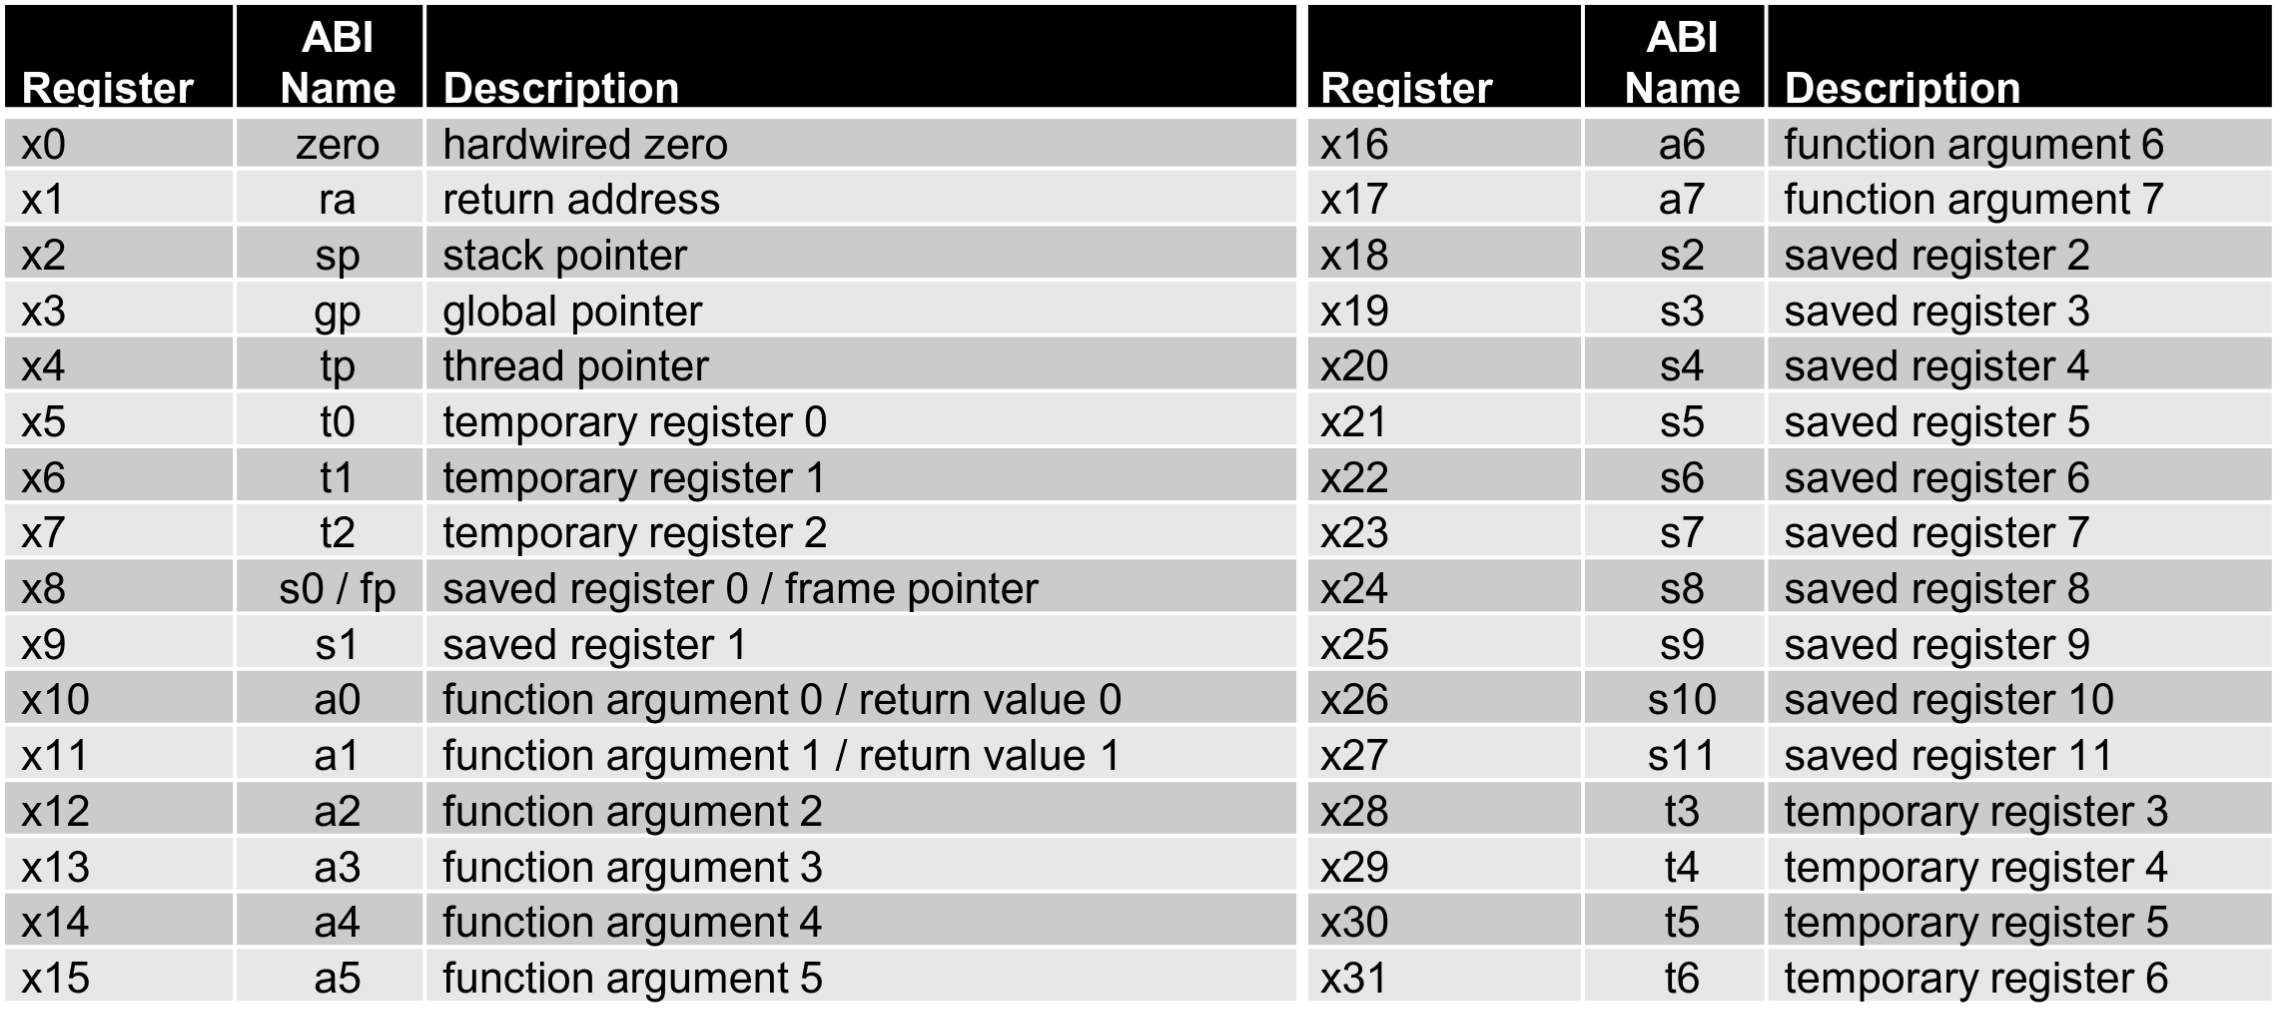
\includegraphics[scale=0.25]{../figures/riscv_reg_abi.png}
\end{figure}

\subsubsection{Addressing modes}

\lstset{language=riscv}

\textbf{Addressing modes} for data transfers are \textit{immediate} and \textit{displacement}, both counting with an encoded field of 12 bits.
\begin{itemize}
	\item \textbf{Immediate} addressing is done through the usual syntax, remembering that we have 3 registers per instruction (destination, source 1 and source 2, as per RISC ABIs): \lstinline|addi x1, x2, 32|;
	\item \textbf{Displacement} is specified on indirect register addressing in load/store instructions: \lstinline|lw x1, 32(x2)|. Let us also note that the \texttt{w} in \lstinline|lw| stands for "word", as in load/store instructions in x86 fashion need their operand size specified in the opcode mnemonic. Of course a displacement of 0 equals to register indirect addressing.
	      An interesting thing is how absolute displacements are specified: we have to include a register for all load instructions, and we can use just the 12 bit displacement as an address if we make that address \texttt{x0} (which we know always evaluates to 0).
\end{itemize}

\subsubsection{Instruction formats}

\textbf{Instruction formats} are an integral part of the RISC-V ABI.
The \textit{green card} available at \url{https://www.cs.sfu.ca/~ashriram/Courses/CS295/assets/notebooks/RISCV/RISCV_CARD.pdf} remains an extremely useful resource.

\begin{center}
	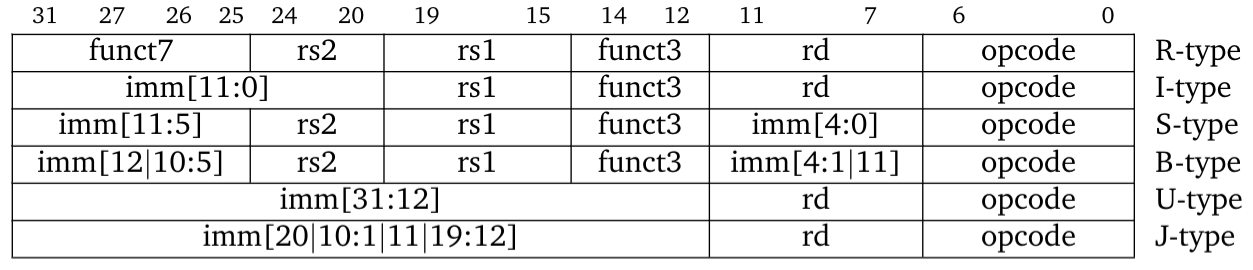
\includegraphics[scale=0.46]{../figures/riscv_types.png}
\end{center}

Each instruction belongs to one of 5 formats, which specifies the semantics of fields within the instruction encoding.
We see that fields like the instruction \textit{opcode}, and the \texttt{funct3} and \texttt{funct7} values are shared between most formats.

\begin{itemize}
	\item \textbf{R-type}: these are \textit{register-to-register} instructions.
	      \begin{table}[H]
		      \center
		      \begin{tabular} { c | p{12cm} }
			      \bfseries Field & \bfseries Decription                                                                                              \\
			      \hline
			      \texttt{opcode} & 7 bit primary operation opcode                                                                                    \\
			      \texttt{rd}     & 5 bit specifier for destination register                                                                          \\
			      \texttt{funct3} & Specifies the type of operation (\lstinline|add| / \lstinline|and| / ...)                                         \\
			      \texttt{rs1}    & 5 bit specifier for first register                                                                                \\
			      \texttt{rs2}    & 5 bit specifier for second register                                                                               \\
			      \texttt{funct7} & Selects a specific suboperation from a main operation (for instance sign extending and non-sign extending shifts) \\
		      \end{tabular}
	      \end{table}

	\item \textbf{I-type}: these are instructions with \textit{immediates}.
	      \begin{table}[H]
		      \center
		      \begin{tabular} { c | p{12cm} }
			      \bfseries Field    & \bfseries Decription                                                                                                                                                                                                                                                   \\
			      \hline
			      \texttt{opcode}    & 7 bit primary operation opcode                                                                                                                                                                                                                                         \\
			      \texttt{rd}        & 5 bit specifier for destination register                                                                                                                                                                                                                               \\
			      \texttt{funct3}    & Specifies the type of operation (\lstinline|addi| / \lstinline|andi| / ...)                                                                                                                                                                                            \\
			      \texttt{rs1}       & 5 bit specifier for first register                                                                                                                                                                                                                                     \\
			      \texttt{immediate} & 12 bit signed immediate used for logical operands, arithmetic signed operands, load/store address byte offsets, and PC-relative branch signed instruction displacement. Note that this is \textit{sign extended}, as all other immediates in RISC-V! (for simplicity). \\
		      \end{tabular}
	      \end{table}

	\item \textbf{S-type}: these are \textit{store} instructions.
	      \begin{table}[H]
		      \center
		      \begin{tabular} { c | p{12cm} }
			      \bfseries Field     & \bfseries Decription                                         \\
			      \hline
			      \texttt{opcode}     & 7 bit primary operation opcode                               \\
			      \texttt{rs1}        & 5 bit specifier for register to add to the 12 bits immediate \\
			      \texttt{rs2}        & 5 bit specifier for register to copy in memory               \\
			      \texttt{funct3}     & Specifies the size of the operation                          \\
			      \texttt{imm} fields & These two values compose the 12-bit signed value.            \\
		      \end{tabular}
	      \end{table}

	\item \textbf{B-type}: these are \textit{branch} (basically conditional additions affecting the program counter) instructions.
	      \begin{table}[H]
		      \center
		      \begin{tabular} { c | p{12cm} }
			      \bfseries Field     & \bfseries Decription                              \\
			      \hline
			      \texttt{opcode}     & 7 bit primary operation opcode                    \\
			      \texttt{rs1}        & 5 bit specifier for first register to compare     \\
			      \texttt{rs2}        & 5 bit specifier for second register to compare    \\
			      \texttt{funct3}     & Specifies the type of comparison                  \\
			      \texttt{imm} fields & These two values compose the 12 bit signed value. \\
		      \end{tabular}
	      \end{table}

	\item \textbf{U-type}: these are so-called \textit{upper immediate} instructions, used to target the upper 20 bits 12 bit immediate instructions can't reach.
	      \begin{table}[H]
		      \center
		      \begin{tabular} { c | p{12cm} }
			      \bfseries Field     & \bfseries Decription                                                   \\
			      \hline
			      \texttt{opcode}     & 7 bit primary operation opcode                                         \\
			      \texttt{rd}         & 5 bit specifier for destination register (usually the program counter) \\
			      \texttt{imm} fields & These two values compose the 20 bit signed value.                      \\
		      \end{tabular}
	      \end{table}

	\item \textbf{J-type}: these are \textit{jump} instructions.
	      \begin{table}[H]
		      \center
		      \begin{tabular} { c | p{12cm} }
			      \bfseries Field     & \bfseries Decription                                                   \\
			      \hline
			      \texttt{opcode}     & 7 bit primary operation opcode                                         \\
			      \texttt{rd}         & 5 bit specifier for destination register (usually the program counter) \\
			      \texttt{imm} fields & These two values compose the 20 bit signed value.                      \\
		      \end{tabular}
	      \end{table}
\end{itemize}

\subsubsection{Available instructions}

The instructions available on the RV32G, grouped by function:
\begin{itemize}
	\item Load and store
	\item ALU operations
	\item Branches and Jumps
	\item Floating Point
	\item Miscellaneous
\end{itemize}
In the following some of the most used instructions and pseudo-instructions are described.

\textbf{\textsf{Load/store}}: as we know, RISC-V processors use a load-store architecture.
The main memory is accessed only through load and store instructions.

\begin{center}
	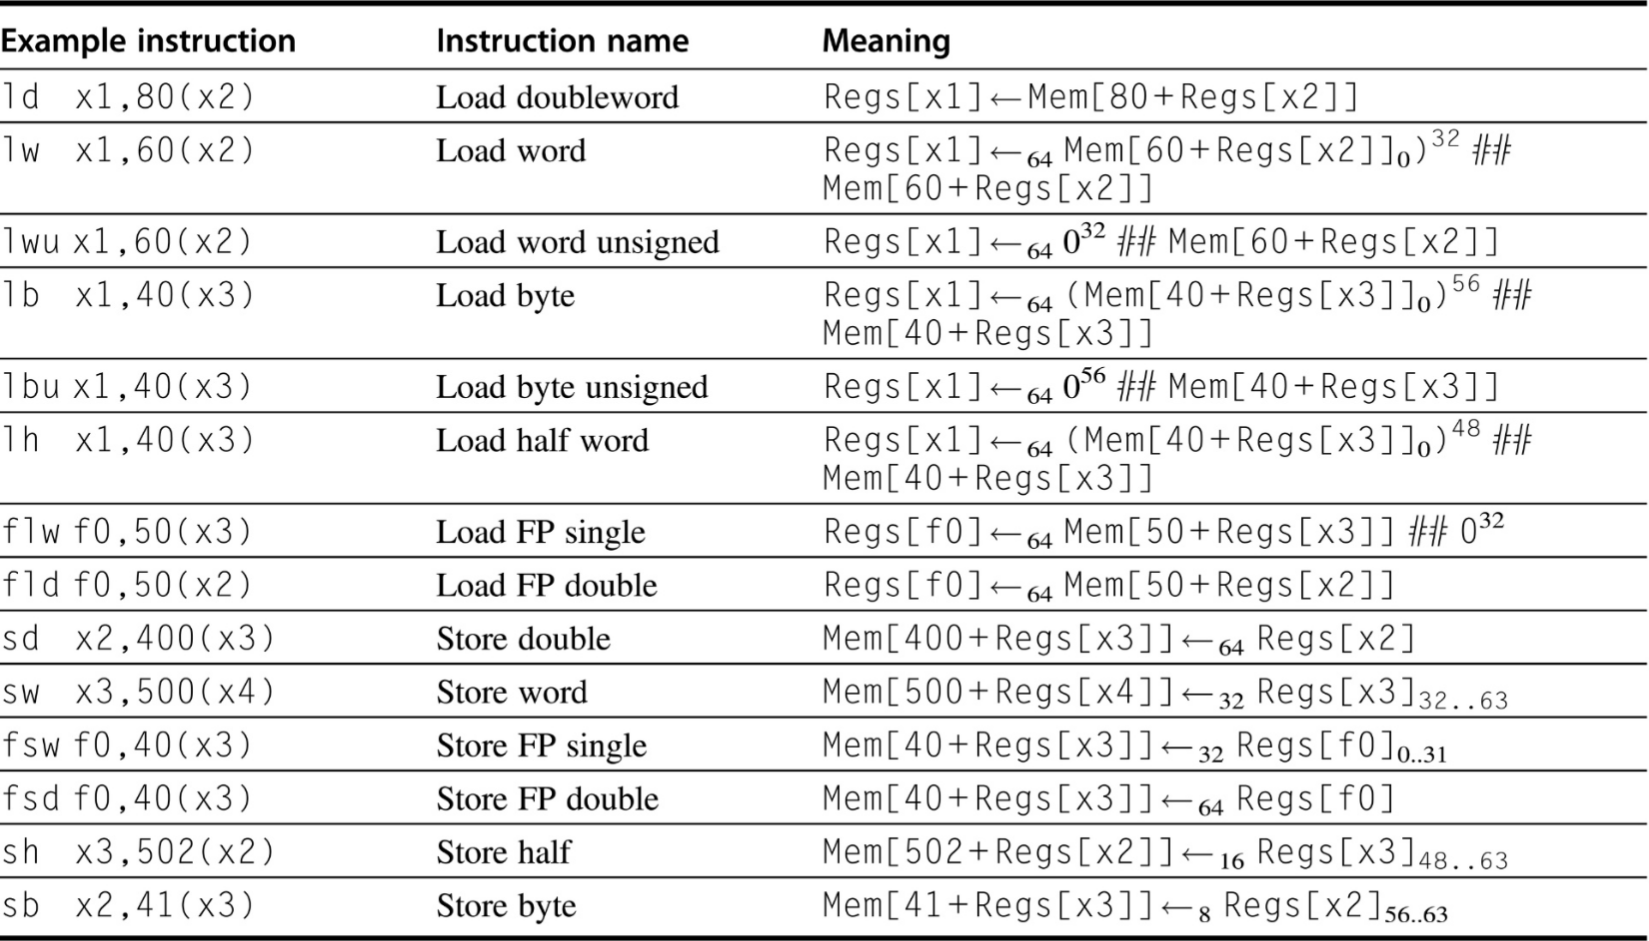
\includegraphics[scale=0.25]{../figures/riscv_load_store.png}
\end{center}

\textbf{\textsf{Pseudo-instructions}} are not actual RISC-V instructions but they are often more convenient for the programmer.
The assembler converts them to real RISC-V instructions (one or more).

One important pseudo-instruction is \lstinline|li|, which stands for \textit{load immediate}.
As we know this operation is not straightforward in RISC-V because immediates are only 12 bits.
\begin{itemize}
	\item For small immediates (which fit into 12 bits) the conversion is straightforward:
	      \begin{lstlisting}[style=codestyle]	
li t0, 4

# translates to:

addi t0, zero, 4
\end{lstlisting}

	\item For big immediates (which don't into 12 bits) the conversion needs an upper immediate instruction:
	      \begin{lstlisting}[style=codestyle]	
li t0, 0xFEDC8765

# translates to:

lui t0, 0xFEDC8    # upper 20 bits
addi t0, t0, 0x765 # lower 12 bits
\end{lstlisting}
\end{itemize}

\textbf{\textsf{ALU operations}} are performed on operands held in the processor registers (we also called them register-to-register operations).

Instruction types are:
\begin{itemize}
	\item Immediate and three-operand instructions;
	\item Shift instructions;
	\item Multiply and divide instructions if the M extension is available.
\end{itemize}

\begin{center}
	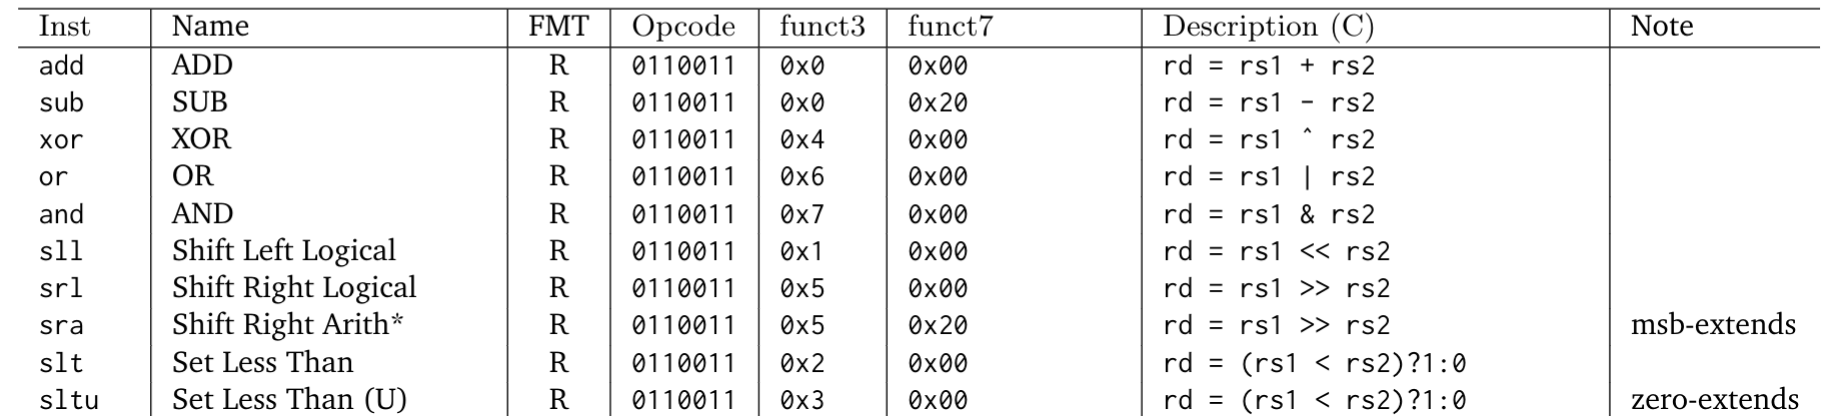
\includegraphics[scale=0.22]{../figures/riscv_alu.png}
\end{center}

Some interesting pseudo-instructions we note are \lstinline|seqz| and \lstinline|snez|:
\begin{itemize}
	\item \lstinline|seqz| sets a destination register if the source register is equal to 0:
	      \begin{lstlisting}[style=codestyle]	
seqz x1,x2

# translates to:

sltiu x1, x2, 1 # if (x2 == 0) x1 <- 1
                # else x1 <- 0
\end{lstlisting}

	\item \lstinline|snez| sets a destination register if the source register is not equal to 0:
	      \begin{lstlisting}[style=codestyle]	
seqz x1,x2

# translates to:

sltu x1, x0, x2 # if (x2 != 0) x1 <- 1
                # else x1 <- 0
\end{lstlisting}
\end{itemize}

\textbf{\textsf{Branches and jumps}}: these comprise control transfer instructions (which are mainly unconditional), including:
\begin{itemize}
	\item  PC-relative jumps;
	\item  Jump to register;
	\item  Conditional branches.
\end{itemize}

\begin{center}
	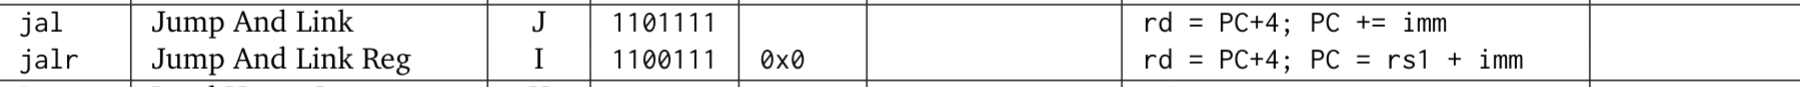
\includegraphics[scale=0.22]{../figures/riscv_jumps.png}
\end{center}

\begin{itemize}
	\item \lstinline|j label|:
	\item \lstinline|jal label|:
	\item \lstinline|jal x3, label|:
	\item \lstinline|jr x3|:
	\item \lstinline|jalr x3|:
	\item \lstinline|jalr x3, x2, 0|:
	\item \lstinline|call sub1|:
	\item \lstinline|ret|:
\end{itemize}

\end{document}
